\documentclass[12pt]{article}
\usepackage{geometry}
\geometry{a4paper}
\usepackage[sort,comma]{natbib}
\usepackage{graphicx}
\usepackage[T1]{fontenc}
\usepackage[utf8]{inputenc}
\usepackage{textcomp}
\usepackage{gensymb}
\usepackage{amsmath}
\usepackage{amssymb}
\usepackage{authblk}
\usepackage[running]{lineno}
\usepackage{setspace}
\usepackage{rotating}
\usepackage{pdflscape}
\usepackage[most]{tcolorbox}

\doublespacing


\title{\large \texttt{insectDisease}: programmatic access to the \textit{Ecological Database of the World's Insect Pathogens}}

\renewcommand\Authfont{\fontsize{12}{14.4}\selectfont}
\renewcommand\Affilfont{\fontsize{10}{10.8}\itshape}

\author[a,b,*]{Tad A Dallas}
\author[c,d]{Colin Carlson} % colin.carlson@georgetown.edu
\author[e,f]{Patrick R Stephens} % prsteph@uga.edu
\author[g, h, i]{Sadie J Ryan} % sjryan@ufl.edu
\author[j]{David W Onstad} % dwonstad@iastate.edu


\affil[a]{Department of Biological Sciences, Louisiana State University, Baton Rouge, LA, 70806}
\affil[b]{Department of Biological Sciences, University of South Carolina, Columbia, SC, 29208}
\affil[c]{Center for Global Health Science and Security, Georgetown University Medical Center, Washington, D.C. 20007}
\affil[d]{Department of Microbiology and Immunology, Georgetown University Medical Center, Washington, D.C. 20007}
\affil[e]{Center for the Ecology if Infectious Disease and Odum School of Ecology, University of Georgia, Athens, GA 30602}
\affil[f]{Department of Integrative Biology, Oklahoma State University, Stillwater, OK 74078}
\affil[g]{ Department of Geography, 3125 Turlington Hall, University of Florida, Gainesville, FL, 32611 USA.}
\affil[h]{Emerging Pathogens Institute, P.O. Box 100009, 2055 Mowry Road, University of Florida, Gainesville, FL 32610 USA.}
\affil[i]{School of Life Sciences, University of KwaZulu-Natal, Private Bag X54001, Durban, 4000, South Africa}
\affil[j]{Corteva Agriscience, Johnston, IA, 50131}




\renewcommand\Authands{ and }
 \date{ \small *Corresponding author: tad.a.dallas@gmail.com}


%%% Target journal
% Ecography (software note) -- maybe we shouldn't re-submit and pay $3000 to publish? 
% Journal of Open Source Software 
% Ecology (data paper)
% 


%%% Potential reviewers
% Lewis Bartlett  lewis.Bartlett@uga.edu UGA
% Philipp Boersch  pboesu@gmail.com   British Trust for Ornithology
% Ben Longdon b.longdon2@exeter.ac.uk Uni of Exeter
% Susan Braxton braxton@illinois.edu U Illinois (could be COI with Onstad though)
% 
% 

%%% Editors
% Thiago Rangel
% 
% 



\begin{document}

\maketitle

\clearpage 
\setstretch{1}

\vspace{-1cm}
\noindent \textbf{Author contributions}: TAD developed the R package, with taxonomic functions developed by CC. All authors contributed to manuscript writing.  \\

\noindent \textbf{Acknowledgements}:  This work was supported by funding to the Viral Emergence Research Initiative (VERENA) consortium including NSF BII 2021909. For more information on the Verena Consortium, see \texttt{https://viralemergence.org}. Earlier development of these data was supported by the Macroecology of Infectious Disease Research Coordination Network (NSF/NIH/USDA DEB 131223). \\

\noindent \textbf{Conflict of interest}: The authors have no conflicts of interest to declare. \\

\noindent \textbf{Keywords}: insect pathogens, crop pest, experimental infection, nematode, virus, protozoa, bacteria  \\



\clearpage
\setstretch{1.35}
\linenumbers




\subsection*{Abstract}
Curated databases of species interactions are instrumental to exploring and understanding the spatial distribution of species and their biotic interactions. In the process of conducting such projects, data development and curation efforts may give rise to a data product with utility beyond the scope of the original work, but which becomes inaccessible over time. Data describing insect host-pathogen interactions are fairly rare, and should thus be preserved and curated with appropriate metadata. Here, we introduce the \texttt{insectDisease} $R$ package, a mechanism for curating, updating, and distributing data from the \textit{Ecological Database of the World's Insect Pathogens}, a database of insect host-pathogen associations, including attempted inoculations and infection outcomes for insect hosts and pathogens (bacteria, fungi, nematodes, protozoans, and viruses). This dataset has been utilized for several projects since its inception, but without a well-defined, curated and permanent repository, its existence and access have been limited to word-of-mouth connections. The current effort presented here aims to provide a means to preserve, augment, and disseminate the database in a documented and versioned format. This project is an example of the type of effort that will be necessary to maintain valuable databases after the original funding disappears.



















\medskip

\noindent \textbf{Running title}: Ecological Database of the World's Insect Pathogens (EDWIP)  \\







 




\clearpage
\setstretch{1.9}
\section*{Introduction}


% the lack of insect disease data
There are a number of data sources documenting host-pathogen associations, especially for pathogens of mammals \citep{gibb2021, patrick2017}, birds \citep{bensch2009}, and fish \citep{fishpest}. Recent work from the Verena Consortium has developed a dynamically updated host-virus association database for all vertebrate hosts (\texttt{VIRION}) \citep{carlson2021}, representing the largest collection of host-virus association data to date. These resources have been fundamental to our understanding of what determines pathogen host range, pathogen species richness across a set of hosts, and overall host-pathogen network structure (e.g, \citet{dallas2018, carlson2020}). But while some host groups are well-studied, there are taxonomic gaps in our understanding of host-pathogen associations. Insect host-pathogen relationships have considerably less open-source data available, despite their inherent importance to scientific studies and assessments of impacts to agricultural crops and spread of vector-borne disease, in addition to the sheer numerical dominance of insect species over other taxa \citep{stork2015}. This is a clear knowledge gap. 




\paragraph*{}
Many of the existing species interaction databases have dedicated researchers, resources, and infrastructure to enable data deposition and curation in openly accessible formats. However, some data have not been as lucky, at no fault of the original data curators. These data run the risk of disappearing into a file drawer or on an external hard drive, potentially shared with a small number of researchers but not accessible to the scientific community at large. One data resource arguably close to this point of disappearance is the \textit{Ecological Database of the World's Insect Pathogens} (EDWIP) \citep{onstad1997}. 



% edwip
\paragraph*{}
The EDWIP data consist of experimental infections and field observations of the interactions between insect hosts and a number of bacterial, fungal, nematode, protozoan, and viral pathogens \citep{braxton2003}. One particularly unique component of EDWIP is the existence of negative associations -- attempts to inoculate a host with a given pathogen that failed to infect -- for some host groups (Figure \ref{fig:bubble}). Failed infections represent \textit{true} absences or incompatibilities between a given host and pathogen. These data are incredibly useful to pathogen host range estimation and host-pathogen interaction modeling, but we rarely have data on these known non-interactions. 


\paragraph*{}
Initially created in 1992, the data have been updated prior to 2000, but no clear semantic versioning was used. As such, it is unclear how long or how frequently this updating and curation continued, and thus, how many different versions of the data may be in existence presently. The database we present here, as the backbone of this R package, represents the most up-to-date version that we know of, though this may differ slightly from previous descriptions of the data \citep{braxton2003}. Generally, we have attempted to preserve all of the original data in the original format.




\subsection*{Solution statement}
To preserve these data in a format that is well-documented, openly accessible, versioned, and flexible for continued development, we created the \texttt{insectDisease} R package. In doing so, we implicitly adhere to the FAIR (Findable, Accessible, Interoperable, Resuable) guidelines for managing data \citep{wilkinson2016}. By hosting the data openly on GitHub, and versioning releases of the data with a permanent identifier (DOI), we ensure the longevity and versioned curation of this data resource. Finally, the incorporation of taxonomic data through \texttt{taxize} \citep{chamberlain2013} ensures that host and pathogen taxonomic names are updated periodically to accommodate for dynamic data or changing taxonomies. 





\subsection*{Data specification}

\paragraph*{Package structure}
Data products are broken down by pathogen group; nematodes (\texttt{data(nematode)}), viruses (\texttt{data(viruses)}), and non-viral pathogens, which include protozoan, fungi, and bacteria (\texttt{data(nvpassoc)}). Data on negative associations is stored collectively instead of being delineated by pathogen group (\texttt{data(negative)}), but information on pathogen group is provided within each of these files, allowing for sorting of negative interactions based on the initial pathogen groupings (Table \ref{tab:data}). This data structure is inherited from the original structure of the EDWIP data files, and code to process and join these different data files is provided in the $R$ package vignette. 



\paragraph*{}
Each of the pathogen groups differs slightly in the available ancillary data on experimental infections. For instance, nematode infections contain information on soil type and associated bacteria, virus infection data have information on viral dose, and non-viral pathogens (protozoans, fungi, and bacteria) have information on intermediate host species. We recommend the user explore these data and associated metadata from within $R$, as the metadata and data are neatly in the same place. 



\paragraph*{}
Data are also available on the insect host species themselves (e.g., \texttt{data(hosts)}). These data contain some information on the Canadian province where the host is found (\texttt{ProvinceI} column), what it eats (\texttt{Food} column), and what type of habitat it is found in (\texttt{Habitat} column). Additionally, a column on host insect pest status is present, offering the opportunity to explore study effort and pathogen specificity dependent on the pest status of the insect host. 




\paragraph*{FAIR data}
The FAIR principles represent guidelines for making data more persistent, findable, and well-documented. Structuring the data as an R package ensures that metadata and data are packaged together, where R manual files contain column names and data descriptions for each data product (\textit{Findable}). All code to take data from the raw data (\texttt{data-raw} folder) to the end product .RData and .csv files is contained in the versioned R data package, and integration with Zenodo (\texttt{https://doi.org/10.5281/zenodo.5821896}) provides a DOI for each release (\textit{Accessible}). Metadata are available in redundant forms, both from within the R package as \texttt{man} files, and in the project README file such that installation of the package (or navigation into the \texttt{man} folder) is not necessary. Apart from providing data in these multiple formats, user access is aided by structuring the data as a package in a very popular computing language among biologists (and other folks too) and providing all code for data processing and serving in an open and public-facing repository (\textit{Interoperable}). Having all code and data in a streamlined, open, and versioned format, serving the data through an interactive web portal, and publishing this software note collectively serve to promote the use of this data resource (\textit{Reusable}).









\paragraph*{Metadata and package documentation}

Differences in features across the data on different pathogen types (e.g., \texttt{?nematodes} relative to \texttt{?viruses}) make combining these data non-straightforward, without a degree of loss of information. We provide some example code in the package \texttt{vignette} on how to go about combining or linking the data across types, with the caveats of information loss, and have standardized some key column names across the different data products. Further, we have documented each data resource using $R$ package documentation, allowing the metadata of each data product to be examined directly from R using the \texttt{help()} function or the question mark notation (e.g., \texttt{?viruses}). These same metadata are also provided in the README file in the top-level of the GitHub repository. 




\paragraph*{Data cleaning and taxonomic resolution}

We attempted to maintain as much of the original data structure from the raw data files provided by David Onstad, principal maintainer of the EDWIP data resource \citep{onstad1997}. This includes files such as \texttt{new\_assoc}, as this was likely a test file containing pathogen species such as ``wormy thing'', and \texttt{newnema}, a dataset identical to \texttt{nematode}. We document these idiosyncrasies in the metadata for each data product, providing a clear overview of the state of each data subproduct. 


\paragraph*{}
The first, and perhaps most important, novel augmentation, is the resolution of host and pathogen taxonomic information. We achieved this by using the R package \texttt{taxize}, specifically the NCBI taxonomic backbone \citep{chamberlain2013}, making the data interoperable with existing data efforts by the Verena Consortium (e.g., VIRION; \citet{carlson2021}). Cached versions of host and pathogen taxonomic information are provided (\texttt{data(hostTaxonomy)} and \\  \texttt{data(pathTaxonomy)}), and the $R$ code to generate these taxonomic backbones and clean the data are provided in the package vignette. This taxonomic backbone serves to both standardize host and pathogen nomenclature, while also correcting any taxonomic changes that have occurred in the past couple decades. This includes the consideration of microsporidian parasites as fungi, not protozoans, a change affecting a large set of records in the EDWIP data. All of the data within the \texttt{data} and \texttt{csv} folders have already gone through these data cleaning steps. However, these data may be dynamic, such that some form of continuous integration or updating of the host and pathogen taxonomy may be necessary. As such, we provide a vignette which transparently shows the steps to clean and augment the data resource, as well as reproduce figures from this manuscript. Finally, we opt to store processed data in the \texttt{csv} folder, which contains all data files in  \texttt{.csv} format. This allows non-$R$ users to access the csv-formatted data easily, and ensures long-term stability of the data, as \texttt{csv} is a stable text file format. These data are also provided as \texttt{.rda} files in the \texttt{data} folder. 



\paragraph*{}
Maintaining the data dynamically as described above allows users to access the data programmatically or as versioned flatfiles (i.e., \texttt{.csv} files). However, for users who do not wish to download the entire data resource, and simply want to quickly query a static version of the database, there is also a standalone web user interface (\texttt{https://edwip.ecology.uga.edu/}) that allows users to easily subset and explore the data. The web interface serves arguably the most important subset of the overall data (data files \texttt{nematode}, \texttt{viruses},\texttt{nvpassoc}, \texttt{negative}, and \texttt{hosts}). This interface allows users to quickly query based on host or parasite taxonomy as a dropdown list. This is perhaps more useful as a teaching tool or for initial exploration of the data, while the programmatic interface and dynamic data may be more useful for more rigorous analysis. This version of the EDWIP data will also only be deployed with a single static copy of the data, such that users wanting to benefit from versioned and dynamic data will need to access the data through the GitHub repository. Future efforts to integrate the web interface and the existing dynamic data structure will be explored, but this is not currently integrated. 








\subsection*{Case study: covariance among pathogen groups in parasite species richness }

Hosts that are infected by more pathogens of one type may also be more infected by pathogens of another type, mediated by host life history traits, metabolic demands, geographic distribution, and intensity of scientific study \citep{dallas2021}. We explore this in the EDWIP data by measuring the number of known positive associations of each of the pathogen groups for each insect host species, visualizing the relationship between the number of pathogens per insect host as a correlation matrix (Figure \ref{fig:corPlot}). We find very little evidence that pathogen groups have positive covariance, which would be expected if host species traits or trait-based sampling biases drove infection process across pathogen groups in the same manner. The failure to detect strong positive relationships, and indeed some negative relationships appearing, could be a signal of the targeted nature of data collection, as many insect host species were selected to study due to their potential as a crop pest, and many pathogens were selected to study based on their potential use as biocontrol or perhaps for their ease of culture. 


\paragraph*{}
This potential sampling bias among insect host species would be evident if there were a positive relationship between the number of positive interactions and the number of negative interactions for a host species, as it would indicate that host species with lots of known interactions also tended to appear in many studies and have some negative interactions as well. We find evidence for a significantly negative relationship based on a Spearman's rank correlation ($\rho$ = -0.1, p $<$ 0.0001), indicating no discernible influence of this relationship. This does not imply that there is no sampling bias in the insect host species researchers opt to study, but that such bias was not so strong as to be clearly detected. 



\subsection*{Concluding comments}

While ecological data are growing in availability, size, accessibility, and stability, there are still data resources that are aging in place, and should not be allowed to fade out of existence. The EDWIP data provided to the authors were in a proprietary format (`Claris FileMaker Pro 5') that was already over 10 major versions behind. With limited inter-version operability (e.g., \texttt{.fmp5} files cannot be opened in more recent versions of the software, or require multiple conversion steps), these data seemed as if headed towards obsolescence. The \texttt{insectDisease} package ensures that these data will be available to the broadest set of researchers, be bound to relevant metadata, and be properly versioned. By hosting the data openly, we welcome contributions from researchers interested in augmenting the data or building off the existing resource. 



\subsection*{Data accessibility}
The \texttt{insectDisease} R package is currently available on GitHub \\ (github.com/viralemergence/insectDisease), with `.csv' files in the csv directory for long-term data stability. GitHub releases of the data ensure versioning is maintained and all versions are accessible. At the time of this writing, the current version is 1.2.0 (available at \\ \texttt{https://github.com/viralemergence/insectDisease/releases/tag/1.2.0}). Releases are given a DOI through integration with Zenodo (\texttt{https://doi.org/10.5281/zenodo.5821896}). 
 















\clearpage
\bibliography{var}
\bibliographystyle{ecography}
\clearpage


























\clearpage

%----------------

\section*{Tables}




\begin{table}[ht]
\centering
\caption{Files associated with the EDWIP data resource. Metadata is stored in $R$ package documentation, allowing the data and metadata to be intrinsically linked. For instance, users can use the help functionality from within $R$ to see more information on data columns and unit (e.g., \texttt{?nematode}). }
\label{tab:data}
\begin{tabular}{cccp{8cm}}
  \hline
  filename & rows & columns & description \\
  \hline
   \texttt{assocref} & 11005  & 16 & references for some host-pathogen associations  \\
   \texttt{citation} & 1966  & 7  & references but no host-pathogen association information  \\
   \texttt{hosts} & 4392  & 21  & insect host trait data\\   
   \texttt{hostTaxonomy} & 4489  & 7  & host taxonomic data updated with the \texttt{getNCBI()} function \\
   \texttt{negative} & 529  & 21  & information on negative host-pathogen associations  \\
   \texttt{nemaref} & 338  & 5  & references from nematode pathogens  \\
   \texttt{nematode} & 234  & 24  & host-nematode interaction data \\   
   \texttt{new\_asso} & 19  & 25  & likely a training document (perhaps do not use)  \\ 
   \texttt{noassref} & 569  & 16  &  references for some host-pathogen associations  \\
   \texttt{nvpassoc} & 7164  & 23  & non-viral pathogen infection data  \\   
   \texttt{pathogen} & 2041  & 9  &  pathogen trait data  \\   
   \texttt{pathTaxonomy} & 2282  & 7  & pathogen taxonomic data updated with the \texttt{getNCBI()} function  \\
   \texttt{viraref} & 2124  & 16  & references from viral infections  \\   
   \texttt{viruses} & 1659  & 25  & host-viral interaction data  \\      
  \hline
\end{tabular}
\end{table}





\clearpage 


\section*{Figures}

\begin{figure}[h!]
  \begin{center}
    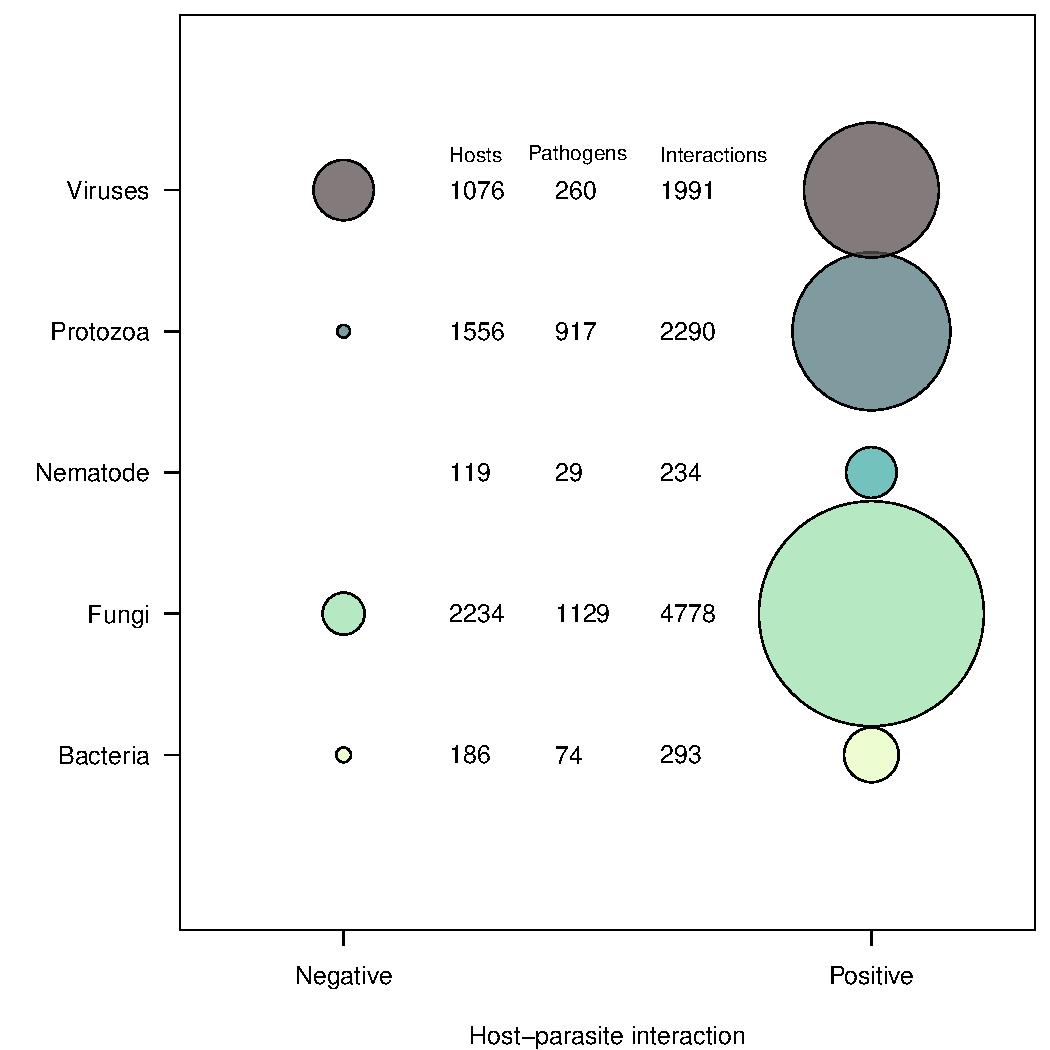
\includegraphics[width=0.85\textwidth]{Figures/bubble.pdf}
    \caption{The number of known non-interactions (\textit{negative} left panel) and known interactions (\textit{positive} right panel) for the set of bacterial, fungal, nematode, protozoan, and viral pathogens ($y$-axis). Bubble size is proportional to the total number of interactions associated with that pathogen group and interaction type (i.e., \textit{negative} or \textit{positive}). Numeric columns correspond to the number of unique host species, pathogen species, and interactions for each pathogen group. }
    \label{fig:bubble}
  \end{center}
\end{figure}




\clearpage


\begin{figure}[h!]
  \begin{center}
    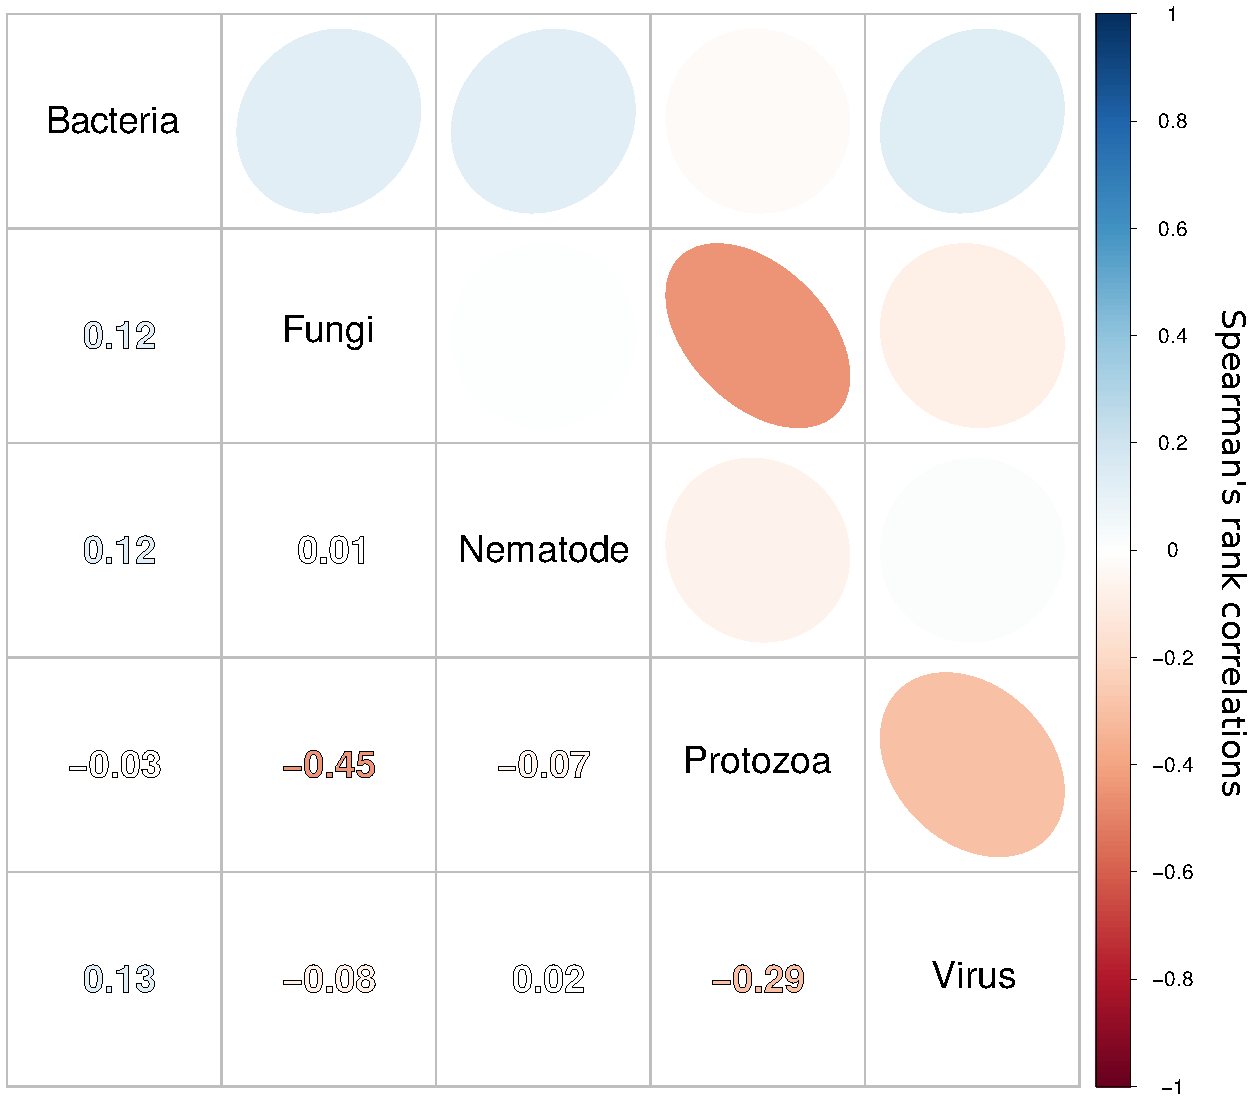
\includegraphics[width=0.8\textwidth]{Figures/corPlot.pdf}
    \caption{Correlations between each pathogen group in terms of pathogen richness of insect host species, where color corresponds to Spearman's rank correlation values (provided in the lower diagonal matrix). Fungal and protozoan pathogens were negatively related, as were viruses and protozoans. Understanding to what extent this is driven by sampling effects or insect host ecology is an outstanding research question that these could be used to begin addressing.}
    \label{fig:corPlot}
  \end{center}
\end{figure}






\end{document}
